%%% prc.tex --- 
%% 
%% Description: 粒子物理与原子核物理实验 作业模板
%% Author: Hongyi Wu(吴鸿毅)
%% Email: wuhongyi@qq.com 
%% Created: 二 9月 22 19:45:13 2015 (+0800)
%% Last-Updated: 二 9月 22 22:08:23 2015 (+0800)
%%           By: Hongyi Wu(吴鸿毅)
%%     Update #: 40
%% URL: http://wuhongyi.cn 

\documentclass[prc,twocolumn,superscriptaddress,showkeys,showpacs,amssymb,amsmath,amsfonts,aps]{revtex4}
\usepackage[slantfont,boldfont]{xeCJK}%中文支持
\usepackage{graphicx} % Required for including pictures
\graphicspath{{Pictures/}} % Specifies the directory where pictures are stored
\usepackage{dcolumn}% Align table columns on decimal point
\usepackage{multirow}%lets you use columns that span multiple rows
\usepackage{epsfig}
\usepackage{latexsym}
\usepackage{amsmath}

%%以下是中文字体的相关设置
\usepackage{indentfirst}% 首行缩进
\setlength{\parindent}{2em}%设置缩进为两个大写M的宽度,大约为两个汉字的宽度
\XeTeXlinebreaklocale "zh"
\XeTeXlinebreakskip = 0pt plus 1pt minus 0.1pt
%字体重命名,方便使用
%% \newfontfamily\times{Times New Roman}
\newCJKfontfamily{\song}{SimSun}
\newCJKfontfamily{\hei}{SimHei}
\newCJKfontfamily{\kai}{KaiTi}
\newCJKfontfamily{\fangsong}{FangSong}
%系统中文查看命令:fc-list :lang=zh
\setmainfont{Times New Roman}%文档正文默认英语字体,设置衬线字体
%% \setsansfont {}%设定无衬线字体
\setCJKmainfont[BoldFont={SimSun},ItalicFont={KaiTi}]{SimSun}%设置默认中文字体
\setCJKsansfont{SimHei}
\setCJKmonofont{FangSong}% 设置等宽字体
%Sans Serif 无衬线字体 楷体、黑体、幼圆 \sansfont 。Serif 衬线字体 对应中文的 宋、仿宋\mainfont
\newcommand{\yihao}{\fontsize{26pt}{26pt}\selectfont} % 一号, 单倍行距
\newcommand{\erhao}{\fontsize{22pt}{22pt}\selectfont} % 二号, 单倍行距
\newcommand{\xiaoer}{\fontsize{18pt}{18pt}\selectfont} % 小二, 单倍行距
\newcommand{\sanhao}{\fontsize{16pt}{16pt}\selectfont} % 三号, 单倍行距
\newcommand{\xiaosan}{\fontsize{15pt}{15pt}\selectfont} % 小三, 单倍行距
\newcommand{\sihao}{\fontsize{14pt}{14pt}\selectfont} % 四号, 单倍行距
\newcommand{\banxiaosi}{\fontsize{13pt}{13pt}\selectfont} % 半小四, 单倍行距
\newcommand{\xiaosi}{\fontsize{12pt}{12pt}\selectfont} % 小四, 单倍行距
\newcommand{\dawuhao}{\fontsize{11.5pt}{11.5pt}\selectfont} % 大五号, 单倍行距
\newcommand{\wuhao}{\fontsize{10.5pt}{10.5pt}\selectfont} % 五号, 单倍行距
\newcommand{\xiaowu}{\fontsize{9.5pt}{9.5pt}\selectfont} % 小五号, 单倍行距
\newcommand{\banbanxiaosi}{\fontsize{12pt}{12pt}\selectfont}% 半半小四, 单倍行距
\defaultfontfeatures{Mapping=tex-text}%如果没有它会有一些tex特殊字符无法正常使用,比如连字符
\XeTeXdefaultencoding"UTF8"
%----------------------------------------------------------------------------------------


\begin{document}

\title{粒子物理与原子核物理实验 作业模板}
\author{吴鸿毅}
\altaffiliation[吴鸿毅: ]{1501110098, wuhongyi@qq.com, (+86)13489853313.}
\affiliation{北京大学物理学院}


\date{\today}% It is always \today, today,
             %  but any date may be explicitly specified

\begin{abstract}
这里是摘要,这里是摘要。这里是摘要,这里是摘要。这里是摘要,这里是摘要。这里是摘要,这里是摘要。这里是摘要,这里是摘要。这里是摘要,这里是摘要。这里是摘要,这里是摘要。这里是摘要,这里是摘要。这里是摘要,这里是摘要。这里是摘要,这里是摘要。\\
这里是摘要,这里是摘要。这里是摘要,这里是摘要。这里是摘要,这里是摘要。这里是摘要,这里是摘要。这里是摘要,这里是摘要。这里是摘要,这里是摘要。这里是摘要,这里是摘要。这里是摘要,这里是摘要。这里是摘要,这里是摘要。这里是摘要,这里是摘要。\\
这里是摘要,这里是摘要。这里是摘要,这里是摘要。这里是摘要,这里是摘要。这里是摘要,这里是摘要。这里是摘要,这里是摘要。这里是摘要,这里是摘要。这里是摘要,这里是摘要。这里是摘要,这里是摘要。这里是摘要,这里是摘要。这里是摘要,这里是摘要。
\end{abstract}
\pacs{23.20.Lv, 25.85.Ca, 21.10.-k, 27.70.+q}% PACS, the Physics and Astronomy Classification Scheme.
\keywords{关键词1, 关键词2, 关键词3, 关键词4}%Use showkeys class option if keyword display desired

\maketitle

\section{引言}%Introduction
实验相关研究领域的背景和现状 (background and status)

有待于研究的实验问题 (question)

为什么要做这个实验?(motivation)

实验的主要内容及创新点(why important and why new)

注意:篇幅不要过长,尽量快速地过度到本实验的研究内容\\

这里是开始。 参考文献引用测试 \cite{Figueredo:2009dg}。这里是正文测试。这里是正文测试。这里是正文测试。这里是正文测试。这里是正文测试。这里是正文测试。

\begin{figure}[h] % Example image
\center{
\includegraphics[width=0.7\linewidth]{placeholder.png}}
\caption{Example image.}
\label{fig:speciation}
\end{figure}



\section{实验}%Experiment
\subsection{实验原理}
这里是正文测试。这里是正文测试。图 \ref{fig:speciation} 这里是正文测试。这里是正文测试。这里是正文测试。这里是正文测试。这里是正文测试。这里是正文测试。这里是正文测试。这里是正文测试。这里是正文测试。这里是正文测试。这里是正文测试。这里是正文测试。这里是正文测试。这里是正文测试。这里是正文测试。这里是正文测试。这里是正文测试。这里是正文测试。这里是正文测试。这里是正文测试。这里是正文测试。这里是正文测试。这里是正文测试。这里是正文测试。这里是正文测试。这里是正文测试。这里是正文测试。这里是正文测试。这里是正文测试。这里是正文测试。这里是正文测试。这里是正文测试。这里是正文测试。这里是正文测试。

\begin{equation}
  \tilde{\beta^{R}} = 1 + \sum_{k=2,4,6...} 2 v_k cos(k\phi_S) \frac{sin(kc)}{kc} R_n \label{Eq:BEff}
\end{equation}
这里是正文测试。这里是正文测试。这里是正文测试。这里是正文测试。这里是正文测试。这里是正文测试。这里是正文测试。这里是正文测试。这里是正文测试。这里是正文测试。这里是正文测试。这里是正文测试。这里是正文测试。这里是正文测试。这里是正文测试。这里是正文测试。公式 (\ref{Eq:BEff}) 明显说明。

\subsection{实验装置图}
探测器(位置,颗粒度,构成等)

放射源,束流

\subsection{实验细节}
尽量列出影响实验结果的条件,如高压,温度,冷却与否,真空与否

这里是正文测试。这里是正文测试。这里是正文测试。这里是正文测试。这里是正文测试。这里是正文测试。这里是正文测试。这里是正文测试。这里是正文测试。这里是正文测试。这里是正文测试。这里是正文测试。这里是正文测试。这里是正文测试。这里是正文测试。这里是正文测试。这里是正文测试。这里是正文测试。
\begin{figure*}[htp]
\begin{center}
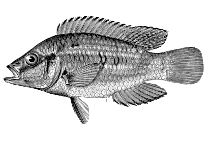
\includegraphics[width=11.5cm]{fish.png}
\vspace{-0.1cm}
\caption{XXXXXXXXXXXXXXXXXXXXXXXXXXXXXXXXXXXXXXXXXXXXXXXXXXXXXXXXXXXXXXXXX} 
\label{isochan}
\end{center}
\end{figure*}
\section{实验结果与讨论}%Experimental results and discussion
列出主要的实验结果
一般需要有数据表\\
一般需要有图。\\
对结果做一定的对比和讨论\\

论据要valid, 论证要reasonable, 结论要convincing.

这里是正文测试。这里是正文测试。这里是正文测试。$a^2+b^2=c^2$ 这里是正文测试。这里是正文测试。这里是正文测试。这里是正文测试。这里是正文测试。这里是正文测试。这里是正文测试。这里是正文测试。这里是正文测试。这里是正文测试。这里是正文测试。这里是正文测试。这里是正文测试。这里是正文测试。这里是正文测试。

分条说明样式:
\begin{itemize}
\item 这里是正文测试。这里是正文测试。这里是正文测试。
\item 这里是正文测试。这里是正文测试。这里是正文测试。这里是正文测试
\item 这里是正文测试。这里是正文测试。
\end{itemize}


\section{总结}%Summary 
这里是正文测试。这里是正文测试。这里是正文测试。这里是正文测试。这里是正文测试。这里是正文测试。这里是正文测试。这里是正文测试。这里是正文测试。这里是正文测试。这里是正文测试。这里是正文测试。这里是正文测试。这里是正文测试。这里是正文测试。这里是正文测试。这里是正文测试。这里是正文测试。这里是正文测试。这里是正文测试。这里是正文测试。这里是正文测试。这里是正文测试。这里是正文测试。这里是正文测试。这里是正文测试。这里是正文测试。这里是正文测试。这里是正文测试。这里是正文测试。这里是正文测试。这里是正文测试。这里是正文测试。这里是正文测试。这里是正文测试。这里是正文测试。表 \ref{varelcoupl} 说明了。
\begin{table}
\caption{Compare of thick and thin target deep-inelastic heavy-ion experiments}
\begin{ruledtabular}
\begin{tabular}{ccc}
                                & Thick target exp. & Thin target exp.  \\      \hline
Doppler correction              & No                & No                \\
Particle detector               & Need't            & Need              \\
Short lifetime $\gamma$-rays    & Can't             & Can               \\
Energy resolution               & Good              & Bad               \\
Radioactive ion beam            & Unsuitable        & Suitable          \\
\end{tabular}
\end{ruledtabular}
\label{varelcoupl}
\end{table}

\section{致谢}%Acknowledge
尊重别人的一种体现\\
可以感谢你的合作者,指导教师,和你讨论对你解释实验数据有所启发的同学等。

这里是正文测试。这里是正文测试。这里是正文测试。
\begin{widetext}
\begin{equation}
 \tilde{v}_n^{R,t} = \frac{v_n+cos(n\phi_S)\frac{sin(nc)}{nc} R_n + \sum_{k=2,4,6...} (v_{k+n}+v_{|k-n|}) cos(k\phi_S) \frac{sin(kc)}{kc} R_n }{1+ \sum_{k=2,4,6...} 2 v_k cos(k \phi_S) \frac{sin(kc)}{kc} R_n}\label{Eq:vnEff}
 \end{equation}
\end{widetext}
这里是正文测试。这里是正文测试。这里是正文测试。这里是正文测试。这里是正文测试。这里是正文测试。
这里是正文测试。这里是正文测试。这里是正文测试。这里是正文测试。这里是正文测试。这里是正文测试。
这里是正文测试。这里是正文测试。这里是正文测试。这里是正文测试。这里是正文测试。这里是正文测试 \cite{Figueredo:2009dg,re111}。

%----------------------------------------------------------------------------------------
%BIBLIOGRAPHY
\bibliography{reference}

\end{document}

%%%%%%%%%%%%%%%%%%%%%%%%%%%%%%%%%%%%%%%%%%%%%%%%%%%%%%%%%%%%%%%%%%%%%%
%%% prc.tex ends here
